\documentclass[10pt, a4paper,titlepage]{article}

\usepackage{graphicx}
\usepackage{tabularx}
\usepackage{listings}
\usepackage[normalem]{ulem}

\begin{document}
\begin{titlepage}
\title{Requirement Analysis and Specification Document \\ Version 1.1}
\author{Emanuele Ricciardelli (mat. 875221) \and Giorgio Tavecchia (mat. 874716) \and Francesco Vetr\'o (mat. 877593)}
\begin{figure}

\includegraphics{/home/francesco/git/Project_SE2_RTV/RASD/RASD_images/logopolimi.png}
\caption{Politecnico di Milano}
\label{fig:logo}
\end{figure}
\maketitle
\end{titlepage}
\tableofcontents
\pagebreak
\section{Introduction}
\subsection{Purpose}
We will project and implement a digital management system for PowerEnJoy, a new car-sharing service. The service is focused on enhancing society's sustainable mobility and a change of mindset from the use of a private property good to a flexible mean of transport based on demand.
The target of this document is to provide a complete and accurate description of the system to be developed, in terms of functional and non-functional requirements that will cover all customer demands. This will lead to a model of the system, represented with the use of different formal languages, useful to manage and achieve development, planning, testing, verification and validation.
This document is intended to users, customers and stakeholders to validate system goals and have an high level description of functionalities, developers and programmers who will implements the system, testers to verify the respect of the requirements and to all other who want an objective description of the system.
\subsection{Scope}
The system should be able to register new users with their credentials, such as name, surname, address and e-mail, their valid driving license number and some payment information. Once the registration process is completed and all entered data are verified, the system will send a password to the user: this password will be used by the user to access the system and its functionalities.
The system provides the following common features:
\begin{itemize}
\item find an available car;
\item reserve an available car one hour prior the pick up;
\item unlock the car when the user is detected nearby the car he/she reserved;
\end{itemize}
In addition there will be incentives for virtuous behaviors of the user that will affect their fares: if an user helps the community by being responsible with the usage of the car, his/her fare will be reduced by a specified percentage; otherwise, by not following the guidelines of the company, the user will be charged more than the standard fare.
\subsection{Goals}
\label{sec:goals}
Users:
\begin{itemize}
\item [{[G1]}] Guest must be able to register himself in the system.
\item [{[G2]}] User must be able to log in and use the system, if registered.
\item [{[G3]}] User must be able to insert a specified address or his current location to find available cars within a certain distance selected by the user himself.
\item [{[G4]}] User must be able to reserve a car for up one hour in advance.
\item [{[G5]}] User must pay a fee of 1 euro if the reserved car is not picked up within an hour from the reservation.
\item [{[G6]}] User must be able to extend his reservation with the payment of a further charge.
\item [{[G7]}] User must be able to notify to the system that he is nearby a reserved car in order to pick it up. 
\item [{[G8]}] User must be able to visualize the current charge of his fare.
\item [{[G9]}] As soon as the engine ignites, the charge is calculated based on the duration of the service.
\item [{[G10]}] User must be notified if his reserved car becomes out of service and it is no longer available.
\item [{[G11]}] User must be able to notify to the company if the reserved car is damaged or not properly working, during their ride or before to pick up the car.
\item [{[G12]}] Users could achieve different discounts if they satisfy different conditions:
\subitem [{G12.1}] 10\% on the last ride if he takes two other passengers with him.
\subitem [{G12.2}] 20\% on the last ride if the car used is left with more than 50\% of the battery.
\subitem [{G12.3}] 30\% on the last ride if the car is parked and left in charge in defined area featured with a power grid.
\item [{[G13]}] It is applied a further 30\% on the ride if the car is parked in one or both of this situations:
\begin{itemize}
\item the car is left at more than 3Km from a power grid
\item the car is left with less than 20\% of the battery.
\end{itemize}
\item[{[G14]}] User must be able to enable a money-saving option.
\end{itemize}
\subsection{Domain properties}
\label{sec:domain}
In the world analysed for the development, we assume the properties defined below:
\begin{itemize}
\item [{[D1]}] All cars available are of the same model.
\item [{[D2]}] When a new car is made available, the company add it to the system.
\item [{[D3]}] When a car is removed from a city either for maintenance or other reasons, the company delete it from the system.
\item [{[D4]}] All the GPS information from a car are always right.
\item [{[D5]}] The GPS of a car can't be switched off, unless the car itself is out of service.
\item [{[D6]}] All information used for identifying how many passengers are in car, are always right.
\item [{[D7]}] Number of passengers is always nonnegative.
\item [{[D8]}] It is always known if the driver is inside the car or not.
\item [{[D9]}] The definition of a parking area to be safe or not is well defined by system.
\item [{[D10]}] The measurement of the battery charge is always correct.
\item [{[D11]}] The maintenance service offered by the company is active 24/7.
\item [{[D12]}] The car locks as soon as the driver close the door and the engine is not running.
\item [{[D13]}] If a user call the maintenance for some problem, a maintainer will show up and always fix the existing problem in less than 2 hours.
\item [{[D14]}] When the maintenance is carrying a car to a safe area, it always choose a the nearest safe area and if the battery charge of the car is less or equal to 80\% then they will choose the nearest one provided with a power grid.
\end{itemize}
\subsection{Glossary}
\begin{description}
\item [Guest] a physical person who access the system for the first time. He/she must provide identification credentials and payment information.
\item [User] he is a user of PowerEnjoy. After the registration, he is defined by the following information:
\begin{itemize}
\item Name
\item Surname
\item Payment information
\item Driving license
\item Password: this attribute is assigned by the system directly at the moment of registration.
\end{itemize}•
\item [Car] it is one of the available cars for the car-sharing service. Each car is identified by:
\begin{itemize}
\item Model (in case of future enlargement of the service provided)
\item License plate
\item Last Driver
\item Number of allowed passengers
\item Availability
\item Percentage of battery
\item GPS position
\end{itemize}
\item [Reserved car] car that has been reserved by one client and will not be available for other reservation until the end of the share.
\item [Ride] represents all the moments starting from the ignition of the engine to the lock of the car at destination.
\item [Driver] is the person who is actually driving the car at a certain moment.
\item [Discount] quantity of money that the driver will not pay for the last drive, based on the characteristics of the ride, passengers and battery usage.
\item [Display] device in the car uses to show information about the car itself and the current ride, like distance, price, discount etc.
\item [Passenger] A passenger is someone who is in the car during a ride but it is not the driver.
\item [Battery bonus] bonus related to the percentage of the car battery left when the user stop renting it.
\item [Passenger bonus] bonus related to the number of passenger who appear in the car during a ride.
\item [Reservation] we say that a car is reserved by an user if the user is not yet in the car but nobody else can take or reserve that car in that moment. Every reservation is defined with an interval of time in which the reservation is preserved and with the data of the user who made it.
\item [Safe area] an area, established by the stakeholders, where a car can be parked to stop the usage and the relative payment. In there, the traffic laws are applied as in normal roads.
\item [Parking area] the meaning is the same of the English one. Some of them could not to be safe areas.
\item [Charging station (alias Power Grid)] area owned by the company that provides plugs to recharge the cars' battery
\item [Plug] physical device that the user or a maintenance person can attach to the car in order to recharge batteries.
\item [Battery] device used to power the car and allows all its functionalities. User can recharge the battery in the charging station but only a maintenance person can access directly the battery itself.
\item [Maintenance person] a physical person that works for the company and whose work is to plug the cars in the electric grid to recharge the batteries if the last driver of the car does not perform this action in a given time, but also provide help to user who face issues during the service and carries cars to a safe area if it is left in an unsafe area.
\item [System] digital management system that will be developed to support the car-sharing service.
\item [Detection zone] geographical area in which the system tries to find an available car
\item [GPS] Global Positioning System, third party artifice that our system use in order to get the position of cars or users.
\item [QR code] image that represent a unique password; the system uses it to guarantee the user the univoque access to the car after a regular reservation
\item [Money Saving option] if selected, the user will be informed on the power grid available near his destination in order to achieve a discount on his ride. With the use of the Money-Saving option, the system ensures a uniform distribution of cars in the city.
\end{description}
\subsection{Text Assumptions}
\begin{itemize}
\item [{[A1]}] We assume that whenever a user damages the rented car or breaks the law regulamentation or isn't able to pay the request fare for the ride, an external association will face the problem of retrieving the amount stated by the company.
\item [{[A2]}] We assume that whenever a user damages a rented car or breaks the law or isn't able to pay the request fare for the ride, he'll be temporary suspended from the service until all the debts will be refund.
\item [{[A3]}] There aren't legacy systems, since the development will provide a brand new service of car-sharing.
\item [{[A4]}] The system generates a specific code when a user reserve a selected car.
\item [{[A5]}] The user receive a code when reserve a car
\item [{[A6]}] The user will apply the valid code on the car. If the code is valid, the car will unlock the doors granting the access to the vehicle.
\item [{[A7]}] Bonuses assumptions
\subitem [{A7.1}] If the system detects that two battery bonuses can be applied for the last ride of an user, only the bonus with the greatest percentage of discount will be applied.
\subitem [{A7.2}] If the system detects that a battery bonus and a passenger bonus are eligible for the last ride of an user, the system will apply the sum of the two.
\subitem [{A7.3}] If the system detects that an user is eligible for a generic bonus and for a malus, the system will apply the sum of the bonus and the malus to the last ride's fare.
\subitem [{A7.4}] If the system detects that an user is eligible for the battery bonus that involves the power grid and a malus, the system will apply only the bonus.
\item [{[A8]}] We assume that if a user leaves a car in an unsafe area, the car will wait 2 minute (to ensure that the driver doesn't plan to enter again) then it will block itself and will notify the system about the current position. A maintenance man will then move the car to a safe area and the last user will be notified for his bad behaviour.
\item [{[A9]}] We assume that, at the end of a ride, the car will be blocked as soon as all driver and passengers are exited the car
\item [{[A10]}] We assume that the system will check, during the registration of a new user, if all the information delivered are correct.
\item [{[A11]}] We assume that the system will implement an algorithm to detect if a user is trying to avoid the correct payment for extending the reservation time. As example: a user is able to extend his reservation further than one hour with the payment of an additional charge. After the reservation has expired, the system will block the user to reserve the same car until at least 30 min are elapsed; if not, the user would be able to pay the fee of 1 euro for expiration time, then reserve again and he will pay a maximum of 1 euro per hour, which will lead to a loss of money for the company.
\item [{[A12]}] We assume that if a car is connected to a power grid until 3 minutes from having parked, the system attributes that the car was put in charge by the last driver.
\item [{[A13]}] We assume that all cars in the system can be seen such as a dumb terminal because they are set of sensors without any kind of logic on it. So, for this reasons, they inform through their sensor the system about the world's situation in which they are and the system reacts based on its own logic.
\item [{[A14]}] \sout{We assume that all cars in the system can be seen such as a dumb terminal because they are set of sensors without any kind of logic on it. So, for this reasons, they inform through their sensor the system about the world's situation in which they are and the system reacts based on its own logic.}
\end{itemize}
\subsection{Constraints}
\subsubsection{Regulatory policies}
\begin{itemize}
\item Privacy policies
\subitem - User position: the system must require the user the permission to get his position in order to indicate the nearest available car. Whenever the user does not allow this permission, the system must ask the user to provide an address for the location of vehicles
\subitem - Car position: the system will provide to the user only the location of the available cars at a certain distance, from a given position.
\item Company policies
\subitem - since the system will use third party artifice and services, e.g. the payment circuit or external help for missing payments, the guests that wants to register to the system and become users needs to accept all the terms proposed by the company with an unilateral agreement
\end{itemize}
\subsubsection{Hardaware limitations}
\begin{itemize}
\item system:
\subitem - user mobile app
\subsubitem . internet connection
\subsubitem . space for app package
\subitem - web application
\subsubitem . modern browser
\item car:
\subitem - GPS
\end{itemize}
\subsubsection{Interface with third party systems}
\begin{itemize}
\item The system will not take care of the payments, since this task will be redirected on the circuit that the user specifies as payment method.
\item Since the service that the system offers is characterized by a high degree of mobility, the system itself will be available for different devices: this implies interfacing with different mobile platforms (android, iOS, etc…)
\item The PowerEnjoy company provides the car-sharing service to a city and high values of state of the art technology characterizes it. Following this idea, the company has stated that owning a physical structures for data, computational power and hosting is unnecessary. Thus we decided to use the rising technology of the cloud thanks to a third party that will be in charge of the maintenance of the system.
\item Car manufacturer produces all the vehicles that are used by the car-sharing service. Figures of reliability and security with respect of passengers are stated by recognized international organization in matter of car security and security of the various electrical systems involved in the car.
\end{itemize}
\subsubsection{Parallel operation}
The system supports simultaneous accesses and requests from different clients.
\subsection{Identifying stakeholders}
The only stakeholder is the company that provides the car-sharing service. The company owns all the car park and provides for maintenance and security. The system-to-be can be easily adapted to other car-sharing services.
\subsection{Reference document}
\begin{itemize}
\item Specification document: Assignments AA 2016-2017.pdf;
\item IEEE Standard for RASD Adapted from ISO/IEC/IEEE 29148 dated December 2011;
\item IEEE Std 830, IEEE Recommended Practice for Software Requirements Specifications;
\item RASD sample from Oct. 20 lecture.pdf
\end{itemize}
\section{Actors identifying}
The actors who take place in our system are:
\begin{itemize}
\item Guest: he is a normal person to access our system in order to registry himself and then become a user.
\item User: he is a person who is registered to the system and is able to reserve and rent all the cars available in PowerEnjoy.
\item Maintenance man: Member of PowerEnjoy delegated to repair vehicles and manage the distribution and the charge of them in the city.
\end{itemize}
\section{Requirements}
\subsection{Functional requirements}
Assuming that all the goals listed in the paragraph \ref{sec:goals} capture all the stakeholders needs, and the domain properties analyzed in \ref{sec:domain} hold, we can derive the following requirements in order to fulfill the goals.
The functional requirements are here grouped under each goal.
\begin{itemize}
\item [{[G1]}] Guest must be able to register himself in the system.
\begin{itemize}
\item The system must be able to check if a guest is already registered.
\item The system must let new user to register only if they are not already registered.
\item The system must verify the payment information.
\item The system must be able to check if the driver license ID is correct.
\item The system must provide a new password to new user to log in.
\end{itemize}
\item [{[G2]}] User must be able to log in and use the system, if registered.
\begin{itemize}
\item The system must be able to check if the password provided is correct.
\item The system must only let the user to login if the provided password is correct.
\item The system must only let logged user to use the functionality of the car-sharing service.
\item The system must save all options selected by a logged user even after the logout.
\end{itemize}
\item [{[G3]}] User must be able to insert a specified address or his current location to find available cars within a certain distance selected by the user himself.
\begin{itemize}
\item The system must be able to detect the user position using information provided by his GPS.
\item The system must be able to receive an input address from the user.
\item The system must be able to detect available cars in a circular area with center in the address provided and radius selected by the user.
\item The system must be able to show to the user the result of the search.
\end{itemize}
\item [{[G4]}] User must be able to reserve a car for up one hour in advance.
\begin{itemize}
\item The system must be able to tag a car as available or reserved.
\item The system must not let other user reserve a car that is already reserved.
\item The system must let the user reserve only a car at a time.
\item The system must let the user able to delete his reservation for free if the cancellation is done before 35 minutes from the reservation, otherwise the cancellation is even possible but the user is charged with 1 euro to face the money loss due to the car's non-usage.
\item The system must associate to every reserved car the user who made the reservation.
\item The system must characterize every reservation with the starting time.
\item The system must be synchronized with the global time. 
\item The system must be able to check if a user has previously reserved the same car.
\item The system must be able to prevent that a user reserves more than one time the same car if the time of the reservation expires with the consequence of paying the related fee.
\end{itemize}
\item [{[G5]}] User must pay a fee of 1 Euro if the reserved car is not picked up within an hour from the reservation.
\begin{itemize}
\item The system must be able to check if the difference between the global time and the starting time of the reservation is greater than the length the reservation, that is initially set to one hour.
\item The system must be able to charge the user who made the reservation if after the length of the reservation the car is not yet picked up.
\item The system must tag the reserved car as “available” after the length of reservation from the starting time, and delete the reservation, if the user who reserved it doesn't show up.
\end{itemize}
\item [{[G6]}] User must be able to extend his reservation with the payment of a further charge.
\begin{itemize}
\item The system must save all data related to reservations for matching them with future reservations.
\item The system must let the user extend his reservation time.
\item The system must not let a user extend a reservation that is not his.
\item The system must further charge the user if he decide to extend his reservation.
\item The system must update the length of the reservation adding the new amount of time (one hour more).
\end{itemize}
\item [{G7}] User must be able to notify to the system that he is nearby a reserved car in order to pick it up. 
\begin{itemize}
\item The system must be able to detect if a user is nearby a car and want to interact with it.
\item The system must let a user access a car if and only if the car has been reserved, to respect of previous condition, by the same user.
\item The system does not allow a user to pick up an unreserved car even if it is available in that moment.
\item The system must be able to notify the user when he tries to unlock a car that he has not reserved.
\end{itemize}
\item [{[G8]}] User must be able to visualize the current charge of his fare.
\begin{itemize}
\item The system must always calculate the charge of a ride.
\item The system must let the user know his current charge.
\end{itemize}
\item [{[G9]}] As soon as the engine ignites, the charge is calculated based on the duration of the service.
\begin{itemize}
\item The system must be able to check if and when a the engine of a car is running.
\item The system must start calculating the charge from the engine ignition.
\item The system must save all information about a ride: driver, number of passengers, duration time, starting position, final position and all information about the car used.
\item The system must able to detect if the car is stopped and no one is on board to stop charging the driver and lock the car.
\item The system must be able to detect if the car is put in charge by the last user or by the maintenance.
\item The system must be able to detect if a car is left in a safe area or not.
\item The system must notify the maintenance if a car is left in an unsafe area and apply a charge to the last driver for the cost of moving the car to a safe area.
\end{itemize}
\item [{[G10]}] User must be notified if his reserved car becomes out of service and it is no longer available.
\begin{itemize}
\item The system must know if a car becomes out of service.
\item The system must save all data related to the malfunctional car.
\item The system must inform the user who reserved a car if the vehicle is no longer available.
\end{itemize}
\item[{[G11]}] User must be able to notify to the company if the reserved car is damaged or not properly working, during their ride or before to pick up the car.
\begin{itemize}
\item The system must let users notify if a car has a problem.
\item The system must notify the maintenance as soon a problem is reported.
\item The system must tag the notified car as out of service as soon as the maintenance ensure the issue.
\item The system must save all data related to an issue.
\item If a user is responsible for some issues on a car, the system must inform an external company to retrieve the money charged to the user.
\item If a user is responsible for some issues on a car, the system will suspend it from the service for a proportional period of time.
\end{itemize}
\item[{[G12]}] Users could achieve different discounts if they satisfy different conditions:
\begin{itemize}
\item The system must know all information about a parked car.
\item The system must know the battery charge of every car.
\item If a car is left with less than 5\% of battery, the system must notify the maintenance to provide the recharge.
\item The system must be able to compute the charge of a ride.
\item The system must apply a discount of 10\% on the last ride if the driver takes at least two other passengers with him.
\item The system must apply the discount related to passengers if and only if the passengers will be on the car during all the ride.
\item The system must apply a discount of 20\% on the last ride if the car used is left with more than 50\% of the battery.
\item The system must apply a discount of 30\% on the last ride if the car is left in charge in a power grid featured area.
\item The system must apply a malus of 30\% on the last ride if the car is left at more than 3KM from a power grid.
\item The system must apply a malus of 30\% on the last ride if the car is left with less than 20\% of the battery.
\item The system must apply only a malus of 30\% even if both above condition are verified.
\item The system must notify the external financial company for every debt of a user.
\item The system must suspend from the service every user who presents some debts towards PowerEnjoy.
\end{itemize}
\item[{[G13]}] User must be able to enable a money-saving option
\begin{itemize}
\item The system must let the user to enable a money-saving option.
\item The system must inform the driver about the nearest available power grid plug to his final destination.
\item The system must know the position of every car and power grid in the city.
\item The system must be able to ensure a uniform distribution of cars in the city.
\end{itemize}
\end{itemize}
\subsection{Non-functional requirements}
\subsubsection{Reliability} 
With respect to cars, availability is proved by car manufacturer that has all the vehicles tested by an international organization. This means that the cars employed for the service is fitted with security devices that are commonly present in any ordinary car. Regarding the system, a first estimation can be given: the system seems to capture the desired requirements and so can be said that all the functionalities will be correct, involving the user operations, the privacy concerns and general correctness. A lot of work will be done in the future, such as developing a correct architecture for the system to allows future improvements, testing and upgrading the system with new functionalities and so on providing a reliability level that is the same or better during the whole system's life.
\subsubsection{Availability}
We can assume that a lower bound for the system availability is set to 99\% on year basis, giving to the company 4 days of tolerance to tackle serious casualties. This parameter is going to be contracted with the third party that owns the computational power and the disks for databases. With respect to the cars, a good maintenance plan is key for not facing problems with availability of the cars themselves.
\subsubsection{Security}
Our system contains sensible data of the users, like the payment information, driving license information and so on. A feasible solution to this problem is to use encryption before storing the sensible data in the system's database and secure communication protocols. Since the payment part of the system is managed by a third party specialized in the field of online payments, we can assume a high protection on the transactions and the money transfer. Another security issue is related to the times of usage: since part of the system, such as cars, and the actions involved, i.e. the reservation and the usage of the car, are disciplined by an external organization (the country and the laws that governs it), the data referred to times of the various actions and the various GPS position must be encrypted as well in order to prevent access to unauthorized third party.
\subsubsection{Maintainability}
The system as whole is composed by two main parts: the cars and the system.
\begin{itemize}
\item cars: maintenance of cars start with a signalization by the user that states that a car is unable to fulfil its duty or by the system that communicates that the state of a car does not respect some required values. The maintenance of the car can evolve in a situation where the car is plugged in the power grid in order to recharge the battery or, if the car has sustained damages, a longer maintenance with the car that is not available for the required time. The maintenance of the car is made by the car manufacturer, so a third party. 
\item system: as stated before, the system will be maintained by the third party operators with respect to the faults that involve hardware part. The maintenance of the software part of the system is our task and it must be addressed everytime an update is found for the developing tools in the future
\end{itemize}
\subsubsection{Portability}
Due to the high degree of mobility of the service, meaning that the user can access the service and so the system in any moment and from every platform, the system will be characterized by:
\begin{itemize}
\item a high degree of portability with respect to the web application, because any modern browser will be able to work as a tool for the user to access the system;
\item a degree of portability with respect to the mobile application that is limited by the different platforms now on the market (e.g. android, iOS, … with all the respecting versions). Since we want to target the largest amount of potential clients, our system will be developed according to the idea that every version of the various platforms will be able to support the system-to-be, with the only constraints regarding the free storage space in the specific device.
\end{itemize}
\section{Scenario identifying}
We will now introduce a set of different scenarios to expose a concrete description of the future features that the system will provide
\subsection{Scenario 1: Registration}
Dilbert lives in a very chaotic city, Gerenzano. He and his family own a station-wagon that is useful during holiday but really difficult to manage in city, in fact finding a parking area is a real nightmare! He knows that different car-sharing service are spreading in the city, in particular he has seen a PowerEnjoy billboard and he's now thinking about giving it a try. He immediately  goes on PowerEnjoy website and reads all the information about the service, ready to register himself. 
He inserts all his anagraphical information, provides his license id and chooses a payment system. It doesn't take too long since he receives an email from PowerEnjoy which confirms his registration and provides him a password to log in in the system.
He is now ready to take advantage to all of PowerEnjoy functionalities.
\subsection{Scenario 2: Reservation of a car}
Batman has an important meeting after works but it will take place on the other side of the city. He knows that, unfortunately,  in the same day it will take place also a strike and so he must be sure to reach his destination on time, right after work.
He decides to reserve a car with PowerEnjoy. It is a very important meeting, so he prefer to pay a little bit more and ensure the car different hours before his departure.
He logs in in the system with his password and then check for an available car near his office, he selects it and confirm the reservation, his new reservation can immediately be found under the "My Reservation" tab; He now moves to it and select the reservation to extend it with the related button. 
He  can now be sure that nobody else will take that car. 
Once exited from his office, he reaches the previous selected car and will unlock it to go to his meeting.
\subsection{Scenario 3: Unlocking a reserved car}
Voldemort has reserved a car because his teleportation device is out of service. So, He leaves his hideout and taking the London's hub, he reaches the reserved car. He opens the PowerEnjoy application on his mobile phone and tap on “my reservation”. The system shows up all the information related to his reservation and provides him the related QR Code. He brings the code on the QR Code reader and the system unlocks the car's doors, noticing to him the success of the operation through a “bip” signal. The reservation's state on the app appears as “picked up”. Finally Voldemort can use his car to reach Hogwarts and destroying Harry Potter.
\subsection{Scenario 4: Hour-expiration fee payment}
Tidus plans to go to a party this evening. Everything is ready and, during diner, Tidus decides to reserve a car with PowerEnjoy to reach the party.
As soon as Tidus leaves his apartment, he meets one of his friend who is directed to the same party and offers him a passage. Tidus accepts it and completely forgot of his reservation with PowerEnjoy!  He knew that he could easily delete his reservation, selecting the "Delete reservation" button under the "My reservation" tab on the app, but now he will be charged, after one hour from the reservation, of 1 Euro for not taking the car.
\subsection{Scenario 5: Deleting a reservation}
Chad Smith has an important concert in Milan this weekend and so, for doing the last preparations, he has decided to reserve a car with the new coolest car-sharing service called PowerEnjoy. 
Unfortunately, a bothering stomachache ruins his plan and he is forced to reschedule his preparations for the next day. He knows that if he doesn't delete his reservation, he'll pay 1 Euro as a fee and even if he is the Red Hot Chili Peppers' drummer and a little fee such that is not a problem, he takes his phone and opens the PowerEnjoy's app. He goes on "My Reservation" tab, his reservation appears and he taps on the "Delete reservation" located on the bottom of the screen. After this, the system notifies him with a message stating the successful result of the operation.
\subsection{Scenario 6: Reserved car becomes out of service}
Mariangiangiangela woke up late today, so she lost the train to go to work and she is afraid to arrive late! She decides to reserve, with the related app on her phone, a PowerEnjoy car that, fortunately, was parked right in front of his house! 
After having breakfast and having dressed, she hears her phone ringing, it is an app-notification which informs her that the car she had reserved, is now out of service! She decides to look out to the balcony and sees a maintenance man who tows the car away! What unfortunate morning.
\subsection{Scenario 7: Car parked in unsafe area}
Pikachu is driving a PowerEnjoy car through the city, going home after a long day of work. He is very tired and as soon he reaches home, he tries to quickly find a parking slot but he is not really caring about parking in a safe area.
So he misses a safe area and end in an unsafe one, not noticing the sign for no parking! He turns off the car and left it, but in this way he will be charged for the wrong parking spot.
As soon as the car blocks itself, the system detects the car's position and reacts by sending a maintenance man who will take care of moving the car to a safe area.
\subsection{Scenario 8: Car put in charge by user, using money saving option}
Dino is having some financial issues in the last month, so he's trying to save some money in everyday life.
For this reason, when he picks up a PowerEnjoy car, he enables the power-saving option! It is very useful because Dino must only insert his final destination and the system provides him a set of nearby power grid in order to put the car in charge after the use and receiving a discount for the virtuous behaviour.
When he reaches a power grid he just exits the car and plug it to the charger. The system, if no more than 3 minutes are elapsed, recognize Dino himself as the one who puts the car in charge and assigns him the discount. Dino is immediately notified by an app-notification for the discount received.
\subsection{Scenario 9: Car found with signs of damage}
Bob is walking down the street and sees from the distance a PowerEnjoy car available, so he decides to take it! But, as soon as he reaches the car, he notices some signs on the body of the car and, knowing that the company could accuse him of the damage if he would use the car without reporting them before, he open his app and selects the "Notify issue" on the main page, he now fulfills a short form providing all necessary information and press the "send" button. The company, after having received the notification, thanks him and quickly send a maintenance man to verify the situation. So now Bob is obliged to research a new car.
\subsection{Scenario 10: User Discounts}
David has been invited at an exclusive party at the Milan's city hall. For reaching the place, David reserves a PowerEnjoy car because his own is out of service. David has read the PowerEnjoy policy when he registered on the website and he knows perfectly what kind of discount the car sharing service has. So he decides to invite two friends of his for splitting the service's costs and mostly for achieving the 10\% discount. When he picks up the car, he notice that the car has been fully charged by the last user, and so he decides to do the same thing for achieving the 30\% discount for plugging the car at the special parking area situated near Palazzo Marino. 
Because of the trip was very short, he also achieves the 20\% discount for leaving the car with more than 50\% of battery full. 
David doesn't know that not all of these discount could be achieved together, but however He is a smart user because (according to the PowerEnjoy's policy) he has saved 10\% due to the passenger bonus and another 30\% due to the recharging operations for a total of 40\% on his last ride's charge.
\subsection{Scenario 11: User bonuses and malus}
Richard has an unlucky day. He reserves a car for reaching his workplace with two other colleagues. Unfortunately they are late and the city center is so congested and so Richard decides to park the car far from the workplace (about 5 kms) and, for not wasting other pricefull time, to take the underground. Unfortunately the underground's stop is not situated near the recharging station and so he doesn't plug in the car, leaving it with less than 80\% of battery charge. The system charges him 30\% more on the last ride fare because of his behavior, according to the company's policy. Nonetheless, he has achieved the 10\% discount for the passenger bonus, so the total charge is not 30\% but only 20\% more on the last ride fare. What an unlucky day!
\subsection{Scenario 12: Nonpayment and suspension from the service}
Ryno is having some problem with his credit card and in particular some payments are resulting loniundone! He discovered it because, trying to reserve a PowerEnjoy car, a popup on the screen notifies him about the suspension from the service until all the past payments will result covered.
\subsection{Scenario 13: Maintenance guy's picking car up}
Donald has reserved a car of the PowerEnjoy car-sharing company. He uses the car for going to the White House, because the PowerEnjoy services are worthy of the U.S. President. He unfortunately hasn't read carefully the policy and he parks and leaves the car in an unsafe area. After three minutes, the system locks the car and notify the maintenance agency to send an employee for carrying it to the nearest safe area. When it's done, the maintenance informs the system that the operation is completed.
\subsection{Scenario 14: Plug-in and unplugged car in a safe area}
Rodd is a maintenance guy of the PowerEnjoy company. Shortly before a rude user has parked his reserved car in a safe area but he has not plugged in the car in the power grid's plug and he left it with less than 5\% of battery level. The system notices that the car is locked, so the user is not allowed to reenter the car, then it notifies the maintenance company. The maintenance sends an employee to plug in the car on the charging station and it informs the system that the operation is completed.
\newpage
\section{UML models}
\subsection{Use case diagram}
\begin{figure}[!h]
\includegraphics[scale=0.5, keepaspectratio]{/home/francesco/git/Project_SE2_RTV/RASD/RASD_images/RASDUML.png}
\caption{Use case diagram}
\label{fig:use case}
\end{figure}
\newpage
\subsection{Use case description}
In this paragraph some of the above use cases will be described.
\begin{table}[h]
\caption{Guest registration} \label{tab:scenario1}
\begin{tabularx}{\textwidth}{|>{\hsize=.4\hsize}X|>{\hsize=.6\hsize}X|}
\hline
Name & Guest register \\
\hline
Actors & Guest \\
\hline
Entry condition & There are no entry conditions. \\
\hline
Flow of events & The guest visits the registration page of the system. \\
& The guest inserts his anagraphical information.\\
& The guest inserts his driver license ID.\\
& The guest selects a payment method.\\
& The guest confirms all data inserted\\
& The system checks the provided information.\\
& The system sends an email to the new user his Password to log in.\\
\hline
Exit conditions & The registration is confirmed and the new user receives his password. \\
\hline
Exceptions & One or more information provided by the guest is incorrect and the system shows an error message, informing the guest to provide valid data and doesn't send any password.\\
\hline
\end{tabularx}
\end{table}
\begin{table}[h]
\caption{User Login} \label{tab:scenario2}
\begin{tabularx}{\textwidth}{|>{\hsize=.4\hsize}X|>{\hsize=.6\hsize}X|}
\hline
Name & User login \\
\hline
Actors & User \\
\hline
Entry condition & There are no entry conditions. \\
\hline
Flow of events & The guest visit the login page of the system. \\
& The guest insert password.\\
& The guest confirm the password inserted.\\
& The system check the password provided.\\
& The system redirect the user to the main page of PowerEnjoy car-sharing service.\\
\hline
Exit conditions & The user is successfully redirected to the main page. \\
\hline
Exceptions & The password provided is not correct and the system doesn't redirect the user to the main page, asking him to enter a valid password.\\
\hline
\end{tabularx}
\end{table}
\begin{table}[h]
\caption{View available cars} \label{tab:scenario3}
\begin{tabularx}{\textwidth}{|>{\hsize=.4\hsize}X|>{\hsize=.6\hsize}X|}
\hline
Name & View available cars \\
\hline
Actors & Logged users \\
\hline
Entry condition & User must be logged and in the main page \\
\hline
Flow of events & The user select to see available cars.\\
& The system redirect him to the related page. \\
& The user select to use GPS position or to insert it manually.\\
& \textit{Alternatively:} \\
& \textit{The system ask the permission to access to GPS position, if available.}\\
& \textit{The user insert the position manually.} \\
& \textit{(end of alternative flow)}\\
& The user confirm the position.\\
& The user select a radius of research.\\
& The system checks all available cars in the designed area.\\
& The system shows all results.\\
\hline
Exit conditions & The page show all available cars in the area designed by the user. \\
\hline
Exceptions & User select to provide GPS information but the system can't access them.\\
& User select an address that is unknown to the system.\\
& In both cases, the system doesn't show any result\\
& and ask to perform again the research.\\
\hline
\end{tabularx}
\end{table}
\begin{table}[h]
\caption{Reservation of a car} \label{tab:scenario4}
\begin{tabularx}{\textwidth}{|>{\hsize=.4\hsize}X|>{\hsize=.6\hsize}X|}
\hline
Name & Reserve a car\\
\hline
Actors & Logged users \\
\hline
Entry condition &  User must be logged and have successfully researched for available cars in an area. \\
\hline
Flow of events & User selects one of the available cars.\\
& The system asks him if he wants to confirm the reservation.\\
& User performs the confirmation.\\
& The system informs the user that he has 1 hour to pick up the car.\\
& The system register the reservation.\\
\hline
Exit conditions & The reservation is confirmed and the user is redirected to the main page. \\
\hline
Exceptions &User select to reserves a car that was available at the beginning of the research but it is now reserved by someone else. In this case the system doesn't confirm the registration and shows an error message.\\
\hline
\end{tabularx}
\end{table}
\begin{table}[h]
\caption{Delete reservation} \label{tab:scenario5}
\begin{tabularx}{\textwidth}{|>{\hsize=.4\hsize}X|>{\hsize=.6\hsize}X|}
\hline
Name & Delete reservation \\
\hline
Actors & Logged users \\
\hline
Entry condition &  User must be logged and in the main page;\\
& user must have performed a reservation that is not yet expired. \\
\hline
Flow of events & User select “manage reservation”.\\
& The system redirects him to the correct page.\\
& The system shows the reservation of the user, with all related information.\\
& The user select to delete the reservation.\\
& The user confirm his decision.\\
& The system delete the reservation.\\
& The system tag the car selected as available\\
& The system charges the user if it is needed according to the company's policy.\\
\hline
Exit conditions & The reservation is deleted, the car available again and the user is redirected to the main page and eventually the user is charged.\\
\hline
Exceptions & There are no exceptions.\\
\hline
\end{tabularx}
\end{table}
\begin{table}[h]
\caption{Extend length of a reservation} \label{tab:scenario6}
\begin{tabularx}{\textwidth}{|>{\hsize=.4\hsize}X|>{\hsize=.6\hsize}X|}
\hline
Name & Extend reservation \\
\hline
Actors & Logged users \\
\hline
Entry condition &  User must be logged and in the main page;\\
& user must have performed a reservation that is not yet expired. \\
\hline
Flow of events & User select “manage reservation”.\\
& The system redirects him to the correct page.\\
& The system shows the reservation of the user, with all related information.\\
& The user select to extend by an hour his reservation.\\
& The user confirm his decision.\\
& The system update the reservation extending its time.\\
& The system charge the user for the extension.\\
\hline
Exit conditions & The reservation  is extended, the user is charged and redirected to the main page.\\
\hline
Exceptions & There are no exceptions.\\
\hline
\end{tabularx}
\end{table}
\begin{table}[h]
\caption{Rent of a car} \label{tab:scenario7}
\begin{tabularx}{\textwidth}{|>{\hsize=.4\hsize}X|>{\hsize=.6\hsize}X|}
\hline
Name & Rent a car \\
\hline
Actors & Logged users \\
\hline
Entry condition &  User must have performed a reservation that is not yet expired. \\
\hline
Flow of events & User reaches his reserved car.\\
& The system detects that the user is providing his reservation code.\\
& The system unlocks the car.\\
& The system detects when the user access the car and the car is ignited.\\
& The system start registering the ride.\\
\hline
Exit conditions & The reservation is completed and the system registers a new ride.\\
\hline
Exceptions & The user is near a car that he has not reserved, the system detects it and notify him. None of the two cars will be unlocked.\\
\hline
\end{tabularx}
\end{table}
\begin{table}[h]
\caption{Money saving option} \label{tab:scenario8}
\begin{tabularx}{\textwidth}{|>{\hsize=.4\hsize}X|>{\hsize=.6\hsize}X|}
\hline
Name & Enable money-saving option \\
\hline
Actors & Logged users \\
\hline
Entry condition & User must have rent a car.\\
\hline
Flow of events & User selects to enable the money-saving option.\\
& The system asks user his destination.\\
& User inserts the destination.\\
& User confirm the destination.\\
& The system provides a set of available power grids near the destination.\\
\hline
Exit conditions & The user is provided by a set of available power grids to plug the car and achieve a discount.\\
\hline
Exceptions & The user insert an invalid destination. In this case the system shows an error message and asks the user to insert a valid address. There aren’t available power grids, in this case the system shows an error message.\\
\hline
\end{tabularx}
\end{table}
\begin{table}[h]
\caption{Report a car's issue} \label{tab:scenario9}
\begin{tabularx}{\textwidth}{|>{\hsize=.4\hsize}X|>{\hsize=.6\hsize}X|}
\hline
Name & Report car’s issue\\
\hline
Actors & Logged users, maintenance system\\ 
\hline
Entry condition & User must have reserved or rent a car and the car must have a problem\\
\hline
Flow of events & User selects to report an issue from the main page\\
& The system redirects him to the related page.\\
& The user inserts a description of the problem.\\
& The system catches the informations of the user’s reservation.\\
& The user confirms the report.\\
& The system redirects him to the main page.\\
& The system notifies the maintenance about the report.\\
\hline
Exit conditions & The issue is reported and the user can leave the car \\
\hline
Exceptions & The user provides an empty description, in this case the system shows an error message and asks to fill the description.\\
\hline
\end{tabularx}
\end{table}
\begin{table}[h]
\caption{Recharge a car} \label{tab:scenario10}
\begin{tabularx}{\textwidth}{|>{\hsize=.4\hsize}X|>{\hsize=.6\hsize}X|}
\hline
Name & Recharge a car\\
\hline
Actors & Logged users\\ 
\hline
Entry condition & User must have rent a car\\
\hline
Flow of events & User exits from the car in a safe area with power grid.\\
& The system locks the car.\\
& The system detects the car's plugging and provides the discount.\\
\hline
Exit conditions & The car is now charging and the user's bill is discounted.\\
\hline
Exceptions & The system doesn’t detect the car’s plugging because the user doesn’t correctly plug the car. In this case the system will not provide the discount to the user and the car will not be recharged.\\
\hline
\end{tabularx}
\end{table}
\begin{table}[h]
\caption{View reported cars by maintenance and selection of one} \label{tab:scenario11}
\begin{tabularx}{\textwidth}{|>{\hsize=.4\hsize}X|>{\hsize=.6\hsize}X|}
\hline
Name & View reported cars\\
\hline
Actors & Maintenance system\\ 
\hline
Entry condition & At least one car has been reported, the maintenance guy is already logged in the system\\
\hline
Flow of events & Maintenance selects the “View reported cars” tab.\\
& The system shows a list of cars reported.\\
& Maintenance selects one of the cars.\\
& The system shows all information about position and reported issue.\\
& The maintenance approves the selection and it handles the situation.\\
& The system update the state of the report as WIP.\\
\hline
Exit conditions & The maintenance goes to the position, the system update the report.\\
\hline
Exceptions & There are no exceptions.\\
\hline
\end{tabularx}
\end{table}
\begin{table}[h]
\caption{Handle a car by maintenance} \label{tab:scenario12}
\begin{tabularx}{\textwidth}{|>{\hsize=.4\hsize}X|>{\hsize=.6\hsize}X|}
\hline
Name & Handle car\\
\hline
Actors & Maintenance guy\\ 
\hline
Entry condition & At least one car has been reported, the maintenance guy is already logged in the system and has selected which cars to work on.\\
\hline
Flow of events & Maintenance goes to the position of the reported cars. Maintenance identifies the problem.\\
& \textit{Alternatively:}\\
& \textit{Maintenance moves the car to the nearest available power grid and plugs the car.}\\
& \textit{Maintenance verifies the damage and take the car away to repair it.}\\
& \textit{Maintenance moves the car, parked in an unsafe area, to a safe area.}\\
& \textit{(end of alternative flow)}\\
& Maintenance notify the system and update the report of the car. The system upgrade the report.\\
\hline
Exit conditions & The report of the issue is updated with information related to the specific intervention.\\
\hline
Exceptions & The maintenance is not able to solve the problem, in this case the system doesn’t update the form and wait to further actions.\\
\hline
\end{tabularx}
\end{table}
\begin{table}[!t]
\caption{Provide a payment} \label{tab:scenario13}
\begin{tabularx}{\textwidth}{|>{\hsize=.4\hsize}X|>{\hsize=.6\hsize}X|}
\hline
Name & Starting payment\\
\hline
Actors & Logged user\\ 
\hline
Entry condition & User has successfully completed a ride and has not payed it yet.\\
\hline
Flow of events & The system elaborates all data related to the ride and computes the charge for the user.\\ 
& The system notifies the user about the charge.\\
& The system notifies the external payment company about the debt of the user.\\
& The system suspends the user from the service until the payment will be performed.\\
& The user provides the payment with the payment system selected during the registration.\\
\hline
Exit conditions & The payment is completed, the external company informs the system and the user is again able to use the functionalities of the car-sharing service.\\
\hline
Exceptions & The payment is not performed: in this case the user remains suspended and the external company provide to stress the user.\\
\hline
\end{tabularx}
\end{table}
\clearpage
\subsection{Class diagram}
\begin{figure}[!h]
\includegraphics[scale=0.4, keepaspectratio]{/home/francesco/git/Project_SE2_RTV/RASD/RASD_images/ClassDiagramCar.png}
\caption{Class Diagram}
\label{fig:Class Diagram}
\end{figure}
\clearpage
\subsection{Sequence diagram}
\begin{figure}[!h]
\includegraphics[scale=0.5, keepaspectratio]{/home/francesco/git/Project_SE2_RTV/RASD/RASD_images/Login.png}
\caption{Sequence Diagram - Login}
\label{fig:Sequence Diagram - Login}
\end{figure}
\clearpage
\begin{figure}[!h]
\includegraphics[scale=0.3, keepaspectratio]{/home/francesco/git/Project_SE2_RTV/RASD/RASD_images/Registration.png}
\caption{Sequence Diagram - Registration}
\label{fig:Sequence Diagram - Registration}
\end{figure}
\clearpage
\begin{figure}[!h]
\includegraphics[scale=0.4, keepaspectratio]{/home/francesco/git/Project_SE2_RTV/RASD/RASD_images/Carreservation.png}
\caption{Sequence Diagram - Car reservation}
\label{fig:Sequence Diagram - Car reservation}
\end{figure}
\clearpage
\begin{figure}[!h]
\includegraphics[scale=0.5, keepaspectratio]{/home/francesco/git/Project_SE2_RTV/RASD/RASD_images/Reportcarissue.png}
\caption{Sequence Diagram - Report car issue}
\label{fig:Sequence Diagram - Report car issue}
\end{figure}
\clearpage
\subsection{Activity diagram}
\begin{figure}[!h]
\includegraphics[scale=0.4, keepaspectratio]{/home/francesco/git/Project_SE2_RTV/RASD/RASD_images/ActivitydiagramPrenotazionecancellazione.png}
\caption{Activity diagram - Prenotazione cancellazione}
\label{fig:Activity diagram - Prenotazione cancellazione}
\end{figure}
\clearpage
\subsection{State diagram}
\begin{figure}[!h]
\includegraphics[scale=0.5, keepaspectratio]{/home/francesco/git/Project_SE2_RTV/RASD/RASD_images/StatediagramCAR.png}
\caption{State diagram - Car}
\label{fig:State diagram - Car}
\end{figure}
\clearpage
\section{Alloy modeling}
\subsection{Model}
\begin{lstlisting}{linewidth=textwidth}
open util/boolean

/**DRAFTS**/
one sig Company{
    cars: set Car,
    map: set SafeArea
}

sig Position{
    latitude: Int,     //should be float
    longitude: Int    //should be float
}

sig Time{
    progressive: Int
}{
    progressive>0
}

one sig ActualTime{
    time : Time
}{
    time.progressive>0
}

sig LicensePlate{}

sig DrivingLicense{}

sig Password{}

sig Code{}

/**AREA**/
abstract sig Area{
    position: Position
}

fact sameAreaSamePosition{
	all a1, a2: Area | (a1.position = a2.position) implies (a1 = a2)
}

sig SafeArea extends Area{}

sig UnsafeArea extends Area{}

/**POWERGRID**/
sig PowerGrid{
           iD: one Int,
           safeArea: one SafeArea,
    chargingCars: set Car,
    capacity: Int
}{
    #chargingCars <= capacity
}

/**CAR**/
sig  Car{
    licensePlate: LicensePlate,
    charge: Int,
    position: Position,
    passengers: Int,
           inCharge : Bool,
           outOfService : Bool,
}{
    charge >= 0 and charge <=100
    passengers > 0 and passengers <= 4
}

/**RESERVATION**/
sig Reservation{
            reservedCar: Car,
            user: User,
            startingTime: Time,
            endingTime: Time,
    unlockingCode: Code
}{
    endingTime.progressive > startingTime.progressive
}

/**USER**/
sig User{
          password : Password,
           suspendedService: Bool,
      drivingLicense: DrivingLicense
}

/**RIDE**/
sig Ride{
     startingPosition: Position,
     endingPosition: Position,
     startingTime: Time,
     endingTime: Time,
     passengers: Int,
     moneySaving: Bool,
    reservation: Reservation,
    charging: lone Charging,
    discount: set Discount
}{
    endingTime.progressive > startingTime.progressive
    startingTime.progressive < reservation.endingTime.progressive
    charging.plugginTime.progressive>endingTime.progressive
    passengers<reservation.reservedCar.passengers and passengers>0
}

/**DISCOUNT**/
//positive value is for malus
//negative value is for bonuses as stated in the document
sig Discount{
    value : Int
}{
    value=30 or value=-10 or value=-20 or value=-30
}

/**CHARGING**/
sig Charging{
   plugginTime: Time,
   powerGrid: PowerGrid   
}

/**DRAFT FACT**/
fact samePosition{
    all p1, p2: Position | (p1.latitude = p2.latitude and 
	p1.longitude = p2.longitude) iff (p1 = p2)
}

fact noLicensePlateWithoutCar{
    all l : LicensePlate | (one c:Car | c.licensePlate=l)
}

fact noPasswordWithoutUser{
    all p:Password | (one u:User | u.password=p)
}

fact noDrivingLicenseWithoutUser{
    all dl:DrivingLicense | (one u:User | u.drivingLicense=dl)
}

fact noCodeWithoutReservation{
	all code: Code | (one res:Reservation| res.unlockingCode=code)
}

/**AREA FACT**/
fact allSafeAreasinMap{
    no s: SafeArea | not (s in Company.map)
}

/**POWERGRID FACT**/
fact onePGChargingOneCar{
    all disjoint pg1, pg2: PowerGrid | (pg1.chargingCars & 
	pg2.chargingCars)=none
}

/**CAR FACT**/
fact uniqueLicensePlate{
    no disjoint c1, c2: Car | c1.licensePlate = c2.licensePlate
}

fact allCarstoCompany{
    no c: Car | not (c in Company.cars)
}

fact noCharginifOutofservice{
    all c: Car | (c.outOfService=True) => (c.inCharge=False)
}

fact ifBatteryLessThan5CarIsOutOfService{ 
    all c: Car| (c.charge<5) implies (c.outOfService=True)
}

fact carInChargingiffPG{
    all car: Car | (car.inCharge=True) iff (one pg:PowerGrid | 
	car in pg.chargingCars and pg.safeArea.position=car.position)
}

fact noChargeThanNoPG{
    all car: Car | (car.inCharge=False) implies
	 (no pg:PowerGrid | car in pg.chargingCars)
}

/**RESERVATION FACT**/
fact noResWithSuspendedService{
    no res:Reservation| res.user.suspendedService=True
}

fact noReservationOnUnavailableCar{
    no r: Reservation | r.reservedCar.outOfService = True
}

fact uniqueReservationPerTimePerUser{
    all disjoint r1,r2 : Reservation, u : User | 
	((r1.user=u) and (r2.user=u)) implies 
	((r1.startingTime!=r2.startingTime) and 
	((r2.startingTime.progressive>r1.endingTime.progressive) or 
	(r1.startingTime.progressive>r2.endingTime.progressive)))
}

fact differentCodeforDifferentReservation{
    no disjoint r1, r2: Reservation | r1.unlockingCode= r2.unlockingCode
}

/**USER FACT**/
fact uniquePassword{
     no disjoint u1,u2: User | u1.password=u2.password
}

fact uniqueDrivingLicense{
    no disjoint u1, u2: User | u1.drivingLicense = u2.drivingLicense
}

/**RIDE FACT**/
fact noUsingCarifinCharge{
	no r: Ride | r.reservation.reservedCar.inCharge=True
}

fact noUsingCarifOutOfService{
    no r: Ride | r.reservation.reservedCar.outOfService=True
}

fact sequentialReservation{
    all res1,res2: Reservation |
    ((res1.reservedCar = res2.reservedCar) => 
	((res1=res2) or 
	(res1.endingTime.progressive <= res2.startingTime.progressive) 
	or 
	(res1.startingTime.progressive >= res2.endingTime.progressive)))
}

fact minus30{
    all ride:Ride | 
	(one disc: Discount| disc.value=-30 and disc in ride.discount) 
		iff (no disc2: Discount | disc2 in ride.discount and 
		(disc2.value=-20 or disc2.value=30))
}

fact minus20{
    all ride:Ride | 
	(one disc: Discount| disc.value=-20 and disc in ride.discount) 
		iff 
		(no disc2: Discount | disc2 in ride.discount and
		(disc2.value=-30))
}

fact minus10{
    all ride:Ride | (one disc: Discount| disc.value=-10 and 
		disc in ride.discount) 
	iff 
	(no disc2: Discount | disc2 in ride.discount and 
	(disc2.value=-30))
}

fact plus30{
    all ride:Ride| (one disc: Discount| 
	disc.value=30 and disc in ride.discount) 
	iff 
	(no disc2: Discount | disc2 in ride.discount and 
	(disc2.value=-20 or disc2.value=-30))
}

fact noSameDiscounts{
	all ride: Ride | 
	(no disjoint d1,d2:Discount | 
		(d1 in ride.discount and d2 in ride.discount 
		and d1.value=d2.value))
}

/**DISCOUNT**/
fact noDiscountWithoutRide{
    all disc : Discount | (one ride : Ride | disc in ride.discount)
}

/**MISC FACT**/
fact RideReservationTime{
    all ride: Ride , res: Reservation | 
	(ride.reservation.reservedCar=res.reservedCar) implies 
		(ride.reservation=res or 
		(res.startingTime.progressive>ride.endingTime.progressive) 
		or
		(res.endingTime.progressive<ride.startingTime.progressive)) 
}

fact noReservationWithMoreRides{
    all res: Reservation, r1,r2: Ride | (r1.reservation=res implies
	(( r2.reservation!=res) or (r1=r2)))
}

fact NoChargingWithoutRide{
    all c:Charging | (one ride: Ride| ride.charging=c)
}

fact ifRideIsJustFinishedCarPositionEqualEndingPosition{
    all r : Ride, c : Car | 
	((r.endingTime=ActualTime.time) and (r.reservation.reservedCar=c))
	 implies (r.endingPosition=c.position)
}



/**ASSERTION**/
assert noUserWithMultipleReservationSimultaneously{
    no disjoint u: User, r1,r2 : Reservation |  
	r1.user=u and r1.user=r2.user 
	and r1.startingTime.progressive=r2.startingTime.progressive
}

assert numberOfPassengersAlwaysLegal{
    no r: Ride | r.passengers>r.reservation.reservedCar.passengers
}

assert noRideIfReservationExpire{
    no ride: Ride | ride.startingTime.progressive>
	ride.reservation.endingTime.progressive
}

assert deletionWithoutFeePayment{
    #Reservation>0 implies 
	(some res:Reservation | res.endingTime.progressive<
		res.startingTime.progressive+35)
}

assert oneDriverPerRide{
    no disjoint u1,u2: User, disjoint r1,r2:Ride | 
	(r1.reservation.user=u1 and r2.reservation.user=u2 and 
	r1.reservation.reservedCar=r2.reservation.reservedCar and
	r1.startingTime.progressive=r2.startingTime.progressive and 
	r1.endingTime.progressive=r2.endingTime.progressive)
}

assert moneySavingOptionAvaliable{
    #Ride>0 implies (some r:Ride | r.moneySaving=True)
}

/**EXECUTION**/

pred show(){}
run show for 5 but 8 Int
check moneySavingOptionAvaliable
check oneDriverPerRide
check deletionWithoutFeePayment
check noRideIfReservationExpire
check numberOfPassengersAlwaysLegal
check noUserWithMultipleReservationSimultaneously
\end{lstlisting}
\subsection{Alloy result}
\textit{
"Check moneySavingOptionAvaliable"
No counterexample found. Assertion may be valid.
\newline
\newline
Executing "Check oneDriverPerRide"
No counterexample found. Assertion may be valid.
\newline
\newline
Executing "Check deletionWithoutFeePayment"
No counterexample found. Assertion may be valid.
\newline
\newline
Executing "Check noRideIfReservationExpire"
No counterexample found. Assertion may be valid.
\newline
\newline
Executing "Check numberOfPassengersAlwaysLegal"
No counterexample found. Assertion may be valid.
\newline
\newline
Executing "Check noUserWithMultipleReservationSimultaneously"
No counterexample found. Assertion may be valid.
\newline
\newline
Executing "Run show for 6 but 8 int"
Instance found. Predicate is consistent.
}
\clearpage
\subsection{World generated}
\begin{figure}[!b]
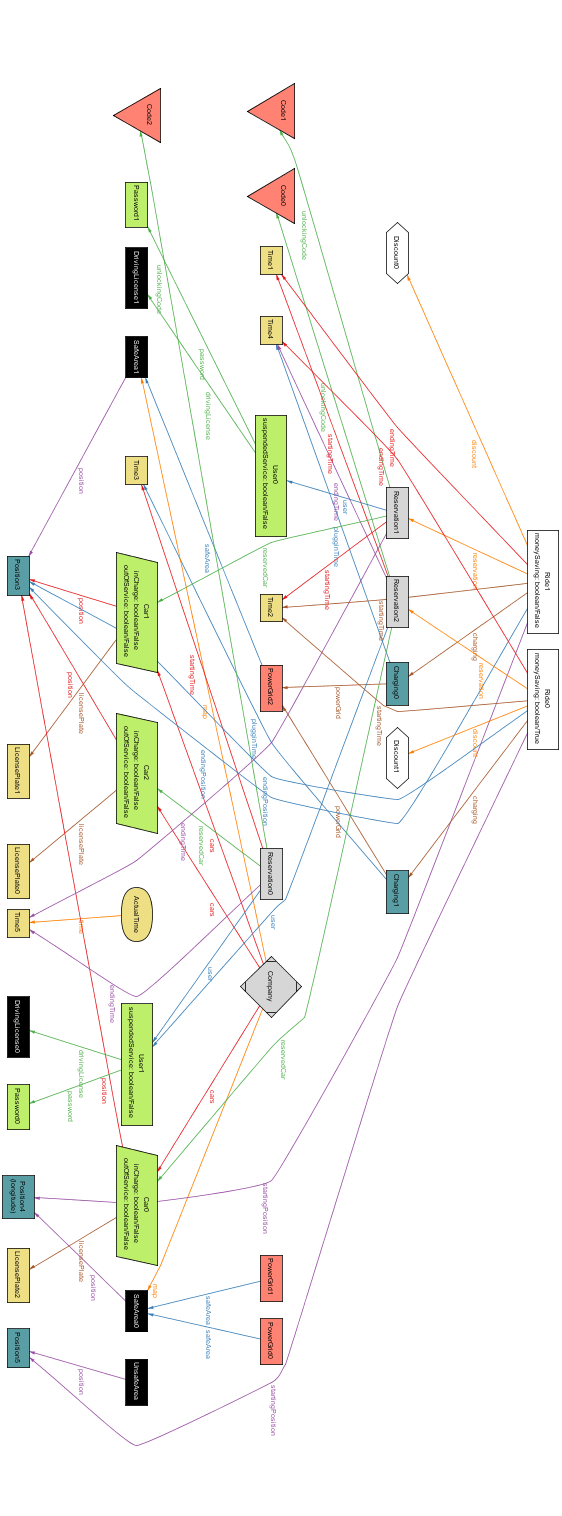
\includegraphics[scale=0.35, keepaspectratio]{/home/francesco/git/Project_SE2_RTV/RASD/RASD_images/screen1.png}
\caption{World generated}
\label{fig:World generated}
\end{figure}
\clearpage
\addcontentsline{toc}{section}{Used tools}
\section*{Used tools}
\begin{itemize}
\item Github: for version control
\item GoogleDoc: to write the document
\item Draw.io: to create the diagrams
\item \LaTeX: to create the pdf
\item Alloy Analizer 4.2: to prove the consistency of our model 
\end{itemize}
\addcontentsline{toc}{section}{Work hours}
\section*{Work hours} 
\begin{itemize}
\item Emanuele Ricciardelli: $\sim$ 34 hrs.
\item Giorgio Tavecchia: $\sim$ 34 hrs.
\item Francesco Vetr\'o: $\sim$ 34 hrs.
\end{itemize}
\addcontentsline{toc}{section}{Changelog}
\section*{Changelog}
\begin{itemize}
\item v1.1
\subitem - [A14] removed because duplication of [A13]
\subitem - modified figure 9: State Diagram - Car
\subitem - fixed layout
\end{itemize}
\end{document}